\documentclass[conference]{IEEEtran}

\usepackage{cite}
\usepackage{amsmath}
\usepackage{graphicx}
\usepackage{fancyvrb}

\begin{document}

\title{Bel's Pyramid Puzzle}

\author{\IEEEauthorblockN{Andrew~Mihal}
\IEEEauthorblockA{Hobbyist\\
Email: andrewcmihal@gmail.com}
\and
\IEEEauthorblockN{Belgacem (Bel) Haba}
\IEEEauthorblockA{Puzzle Enthusiast\\
Email: all4dz@gmail.com}
}

\maketitle

\begin{abstract}
Bel's Pyramid is a recreational mathematics puzzle involving stacking cubes to create a square step pyramid,
under the constraint that adjacent cube faces must have the same label.
Solutions for pyramid sizes up to $N=5$ are currently known.
We propose a collection of SAT benchmarks that solve this puzzle for various configurations,
including variations on the SAT encoding, different symmetry-breaking strategies, and proofs
that some constructive solutions are infeasible.
\end{abstract}

\section{Problem Description}
Bel's Pyramid is a cube-stacking puzzle invented by the co-author.
The goal is to create a square step pyramid with $N$ levels using a set of uniquely-labelled cubes.
Cube faces that touch must have the same label.
The cubes are labeled in a special way that is detailed below.

It is hypothesized that multiple solutions exist for every puzzle size $N$, but as of this writing there is no known
constructive approach for generating any solution for an arbitrary $N$.
All known solutions for non-trivial puzzles have been discovered using search (specifically SAT).
SAT has also been able to prove that some proposed constructive approaches are infeasible.
The end goal is to find a general solution.

\begin{figure}[htbp]
\centerline{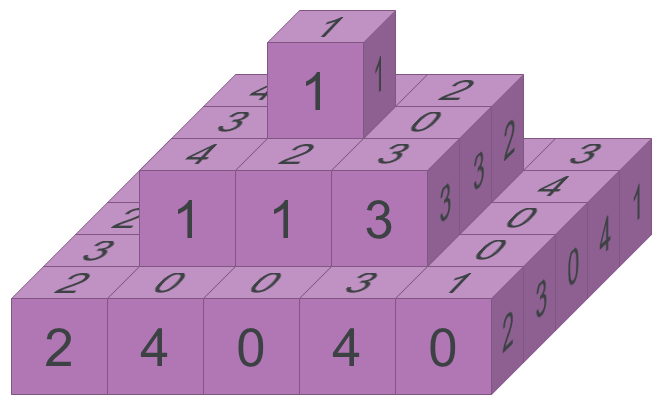
\includegraphics[width=\linewidth]{example.png}}
\caption{Solved $N=3$ Pyramid}
\label{example}
\end{figure}

Figure~\ref{example} shows the geometry of a solved pyramid with $N=3$ layers.
Each layer $n\in[0,N)$ is a square with side length $2n+1$.
The layers are aligned vertically along their center cubes to create a symmetric step pyramid. The total number of cubes in the pyramid is:

\begin{equation}
\sum_{n=0}^{N-1}(2n+1)^2 = \frac{1}{3}N(4N^2-1)
\end{equation}

\subsection{Cube Labels}

The cubes have labels on each of their faces, and importantly, cubes always have the same label on opposite faces.
In a pyramid with $N$ layers there are $2N-1$ distinct labels.
Each cube has a unique labelling $(a,b,c)$ which is generated by choosing 3 labels from the set of $2N-1$ \emph{with replacement}.
The number of possible combinations with replacement is identical to the number of cubes:

\begin{equation}
\begin{aligned}
\left(\binom{2N-1}{3}\right) &= \binom{(2N-1)+3-1}{3} \\
&= \frac{1}{3}N(2N-1)(2N+1) \\
&= \frac{1}{3}N(4N^2-1)
\end{aligned}
\end{equation}

Note that a permutation of the label tuple $(a,b,c)$, e.g. $(c,a,b)$, corresponds to a spatial rotation of a cube and is not a separate cube.
Cubes have up to 3 distinct labels and 6 possible rotations.
Cubes with repeated labels have fewer distinguishable rotations.
Each cube is unique and must be used exactly once to solve the pyramid.
Cubes can be placed into the pyramid with any rotation.

\subsection{Axis Labels}

Due to the rule that opposite cube faces have identical labels, any line of cubes along an axis must have the same label all the way down the axis.
Therefore one does not need to see the hidden faces to determine the state of the pyramid.
It is only necessary to see the labels on the top, front, and right external faces.

A solution can be written in a compact ASCII-art format, suggested by Donald Knuth, that is reminiscent of an architect's elevation drawing.
The solution for the same pyramid in Figure~\ref{example} is as follows:

\begin{center}
\begin{small}
\begin{BVerbatim}
+----------------+
|  2  1  1  4  3 |  1
|  2  4  1  2  4 |  4  2
|  2  3  1  0  0 |  0  3  1
|  3  4  2  3  0 |  3  3
|  2  0  0  3  1 |  2
+----------------+
   2  4  0  4  0
      1  1  3
         1
\end{BVerbatim}
\end{small}
\end{center}

The labels on three orthogonal external faces determine the specific cube and rotation at the intersection point of the axes through those faces.
Conversely, placing a cube at a specific location determines three orthogonal axis labels.
Doing either of these things further constrains the cubes that can be placed along the same axis lines.

\section{SAT Encoding}

A solver implemented with Z3Py~\cite{z3} is available at~\cite{b1}.
The constraint formulation uses bounded integer variables (or optionally enumeration sorts) for the axis label assignments,
and Boolean variables to indicate that a specific cube is placed at a certain coordinate with a certain rotation.
There are only two types of constraints: a cube uniqueness constraint asserts that each cube must be placed at exactly one coordinate with one rotation.
This is an exactly\nobreakdash-1 cardinality constraint over the Boolean placement variables for each cube.
The second type of constraint asserts that a conjunction of three orthogonal axis assignments is equivalent to one of the Boolean placement variables.

The Python program is capable of exporting the problem in CNF or SMT2 format.
It can also re-import certificates to print and verify solutions generated by an external solver.
The program has options documented on the gitHub page for applying different Z3 solver tactics and symmetry-breaking strategies.

\section{Constructive Solutions}

An algorithmic process for constructing solutions for any pyramid size $N$ is not currently known.
It is tempting to seek a recursive process that uses the solution for an $N-1$ pyramid to solve the $N$ pyramid quickly.
Two such proposals are given below, and SAT can be used to easily show that they do not generalize.

\subsection{Adding a New Base Layer}

The ``new base layer'' approach takes a solved pyramid with $N-1$ layers and adds the next layer of size $(2N-1)\times(2N-1)$ underneath it.
An $N$\nobreakdash-layer pyramid has two additional labels compared to an $N-1$ pyramid.
All of the cubes with the two new labels must be located on the new bottom layer.
The same property applies for each layer up to the top of the pyramid, which must be the trivial $N=1$ subproblem with the single cube $(0,0,0)$.
This recursive approach works only for $N$ up to 3 and is UNSAT for $N=4$, proving that this strategy cannot be the basis of a generic solution.

\subsection{Adding a New Top Shell}

This approach takes a solved $N-1$ pyramid and drops an additional layer of cubes on top of it to create a $N$\nobreakdash-layer pyramid.
All of the cubes with the two new labels are on top of the pyramid, wrapping around the previous pyramid.
The trivial $(0,0,0)$ pyramid is at the center of the bottom layer.
This approach also only works for $N$ up to 3.

\section{Symmetry-Breaking Strategies}

The puzzle has various geometric symmetries and is also symmetric under permutations of the labels.
The solver program has options to apply additional constraints to break some of these symmetries.

\begin{itemize}
\item The label permutation symmetry can be broken by adding lexicographical ordering constraints on the axis label variables.
The axis labels can be constrained left-right, top-down as one would read the solution.
Heuristic importance can also be considered.
Labels on the longest axes control the most number of cubes and may hypothetically benefit from more constrained assignments to limit the search space.
\item Mirroring and rotation geometric symmetries can be also be broken by applying ordering constraints between pairs of axis label
variables on the front and right faces of the pyramid.
There is an additional geometric symmetry that allows entire vertical slices of the pyramid on opposite sides of the centerline to be
swapped without affecting any other cubes.
This one can be broken with ordering constraints between pairs of axis labels on the same face of the pyramid.
\item A few types of lookahead constraints are considered to prevent the seach from exploring subspaces where too many axes have been
assigned to the same label, such that there aren't enough blocks with that label to fill all of the spaces along those axes.
\item In addition to the infeasible recursive constructive strategies described earlier, there are also options for \emph{partial} constructive strategies
that don't build on independently solved subproblems.
These strategies place or constrain some blocks, or assign or constrain some axis labels, and then use SAT to try to solve the rest of the pyramid.
Often they are based on intuition or informal geometric patterns in the hope of yielding insight towards a general solution.
None have yet been successful.
\end{itemize}

\section{Results}

$N=4$ pyramids can be solved by Kissat~\cite{k1} in less than a minute.
$N=5$ pyramids with partial constructive strategies to limit the search space take on the order of ten minutes.
Even with the fastest known combination of strategies, no $N=6$ pyramid has yet been solved.
Up to a week of runtime using ParKissat-RS on a 32-thread machine has been attempted.

The proposed benchmarks use combinations of pyramid sizes and symmetry-breaking strategies to provide variations in difficulty in the one-to-ten minute range.
UNSAT instances that disprove a selection of recursive constructive strategies are also included.

\begin{thebibliography}{0}
\bibitem{b1} A. Mihal. ``Bel's Pyramid Puzzle,'' 2025, gitHub repository. [Online]. Available: https://github.com/acmihal/bel\_pyramid
\bibitem{z3} L. De Moura and N. Bj{\o}rner. ``Z3: An Efficient SMT Solver,'' In TACAS'08. 337--340
\bibitem{k1} A. Biere et al. ``CaDiCaL, Gimsatul, IsaSAT and Kissat Entering the SAT Competition 2024''. In Proc. SAT Comp. 2024. 8--10
\end{thebibliography}

\end{document}
